\documentclass{beamer}

\usepackage{beamerthemeuzbl}
\usepackage{listings}
%\usepackage{beamerthemeCambridgeUS}
\title{Uzbl - web interface tools which adhere to the unix philosophy}
\author{Dieter Plaetinck}
\date{06-02-2010}
\begin{document}
%\mbox{}\vfill
%\vspace*{\fill}
%\mbox{}
%\vspace{10 mm}
%\vspace*{14mm}
\begin{center}

\includegraphics[scale=2.2]{logo3.png} % to show when not talking
\end{center}
%\vfill
\frame{\titlepage}

\section[Outline]{}

\section{Introduction}

\frame{
\LARGE 
\begin{center}The unix philosophy.\end{center}
}
% different interpretations
% programs that do one thing & well. work together. plain text = universal

% my goal: all apps on my desktop to adhere to it.
% i want: building blocks, integration. control & reuse my own data.

\frame{
\frametitle{Examples} %anyone using this?
\begin{itemize}
\large
\item mpd
\item dmenu
\item awesome/xmonad/dwm/wmii/...
\item dzen
\item zenity
\item bitlbee
\item mplayer/vlc (without GUI)
\item bashrun
\end{itemize}
}

\definecolor{light-gray}{gray}{0.95}
\subsection{Everyone likes stats...} % go over each very quickly
\frame
{
  \frametitle{Stats}

  \begin{itemize}
\large
  \item start april 2k9
  \item 60 contributors % just counting git. not ML or wiki
  \item 11k LOC % 5k C "core" stuff, 5k sloc python % example scripts, browser, tabbed. 1k of sh and js
  \item 13 releases % release early, release often.
  \item 100 scripts % 20 scripts in our repo, 70 on wiki, about 10 websites
  \end{itemize}
}

\lstset{breaklines=true,numbers=none,backgroundcolor=\color{light-gray},basicstyle=\footnotesize}

\subsection{Uzbl}
\frame
{
\frametitle{Uzbl?}
  \begin{itemize} %very briefly explain each
\Large
  \item uzbl-core % meant for integration, extend with scripts
  \item uzbl-browser % fullfeatured browser based on uzbl-core
  \item uzbl-tabbed 
  \item ... % whatever you want: feed reader, presentation tool, in emacs: ezbl
  \end{itemize}
}

\section{Uzbl-core}
\frame
{
\frametitle{Uzbl-core} 
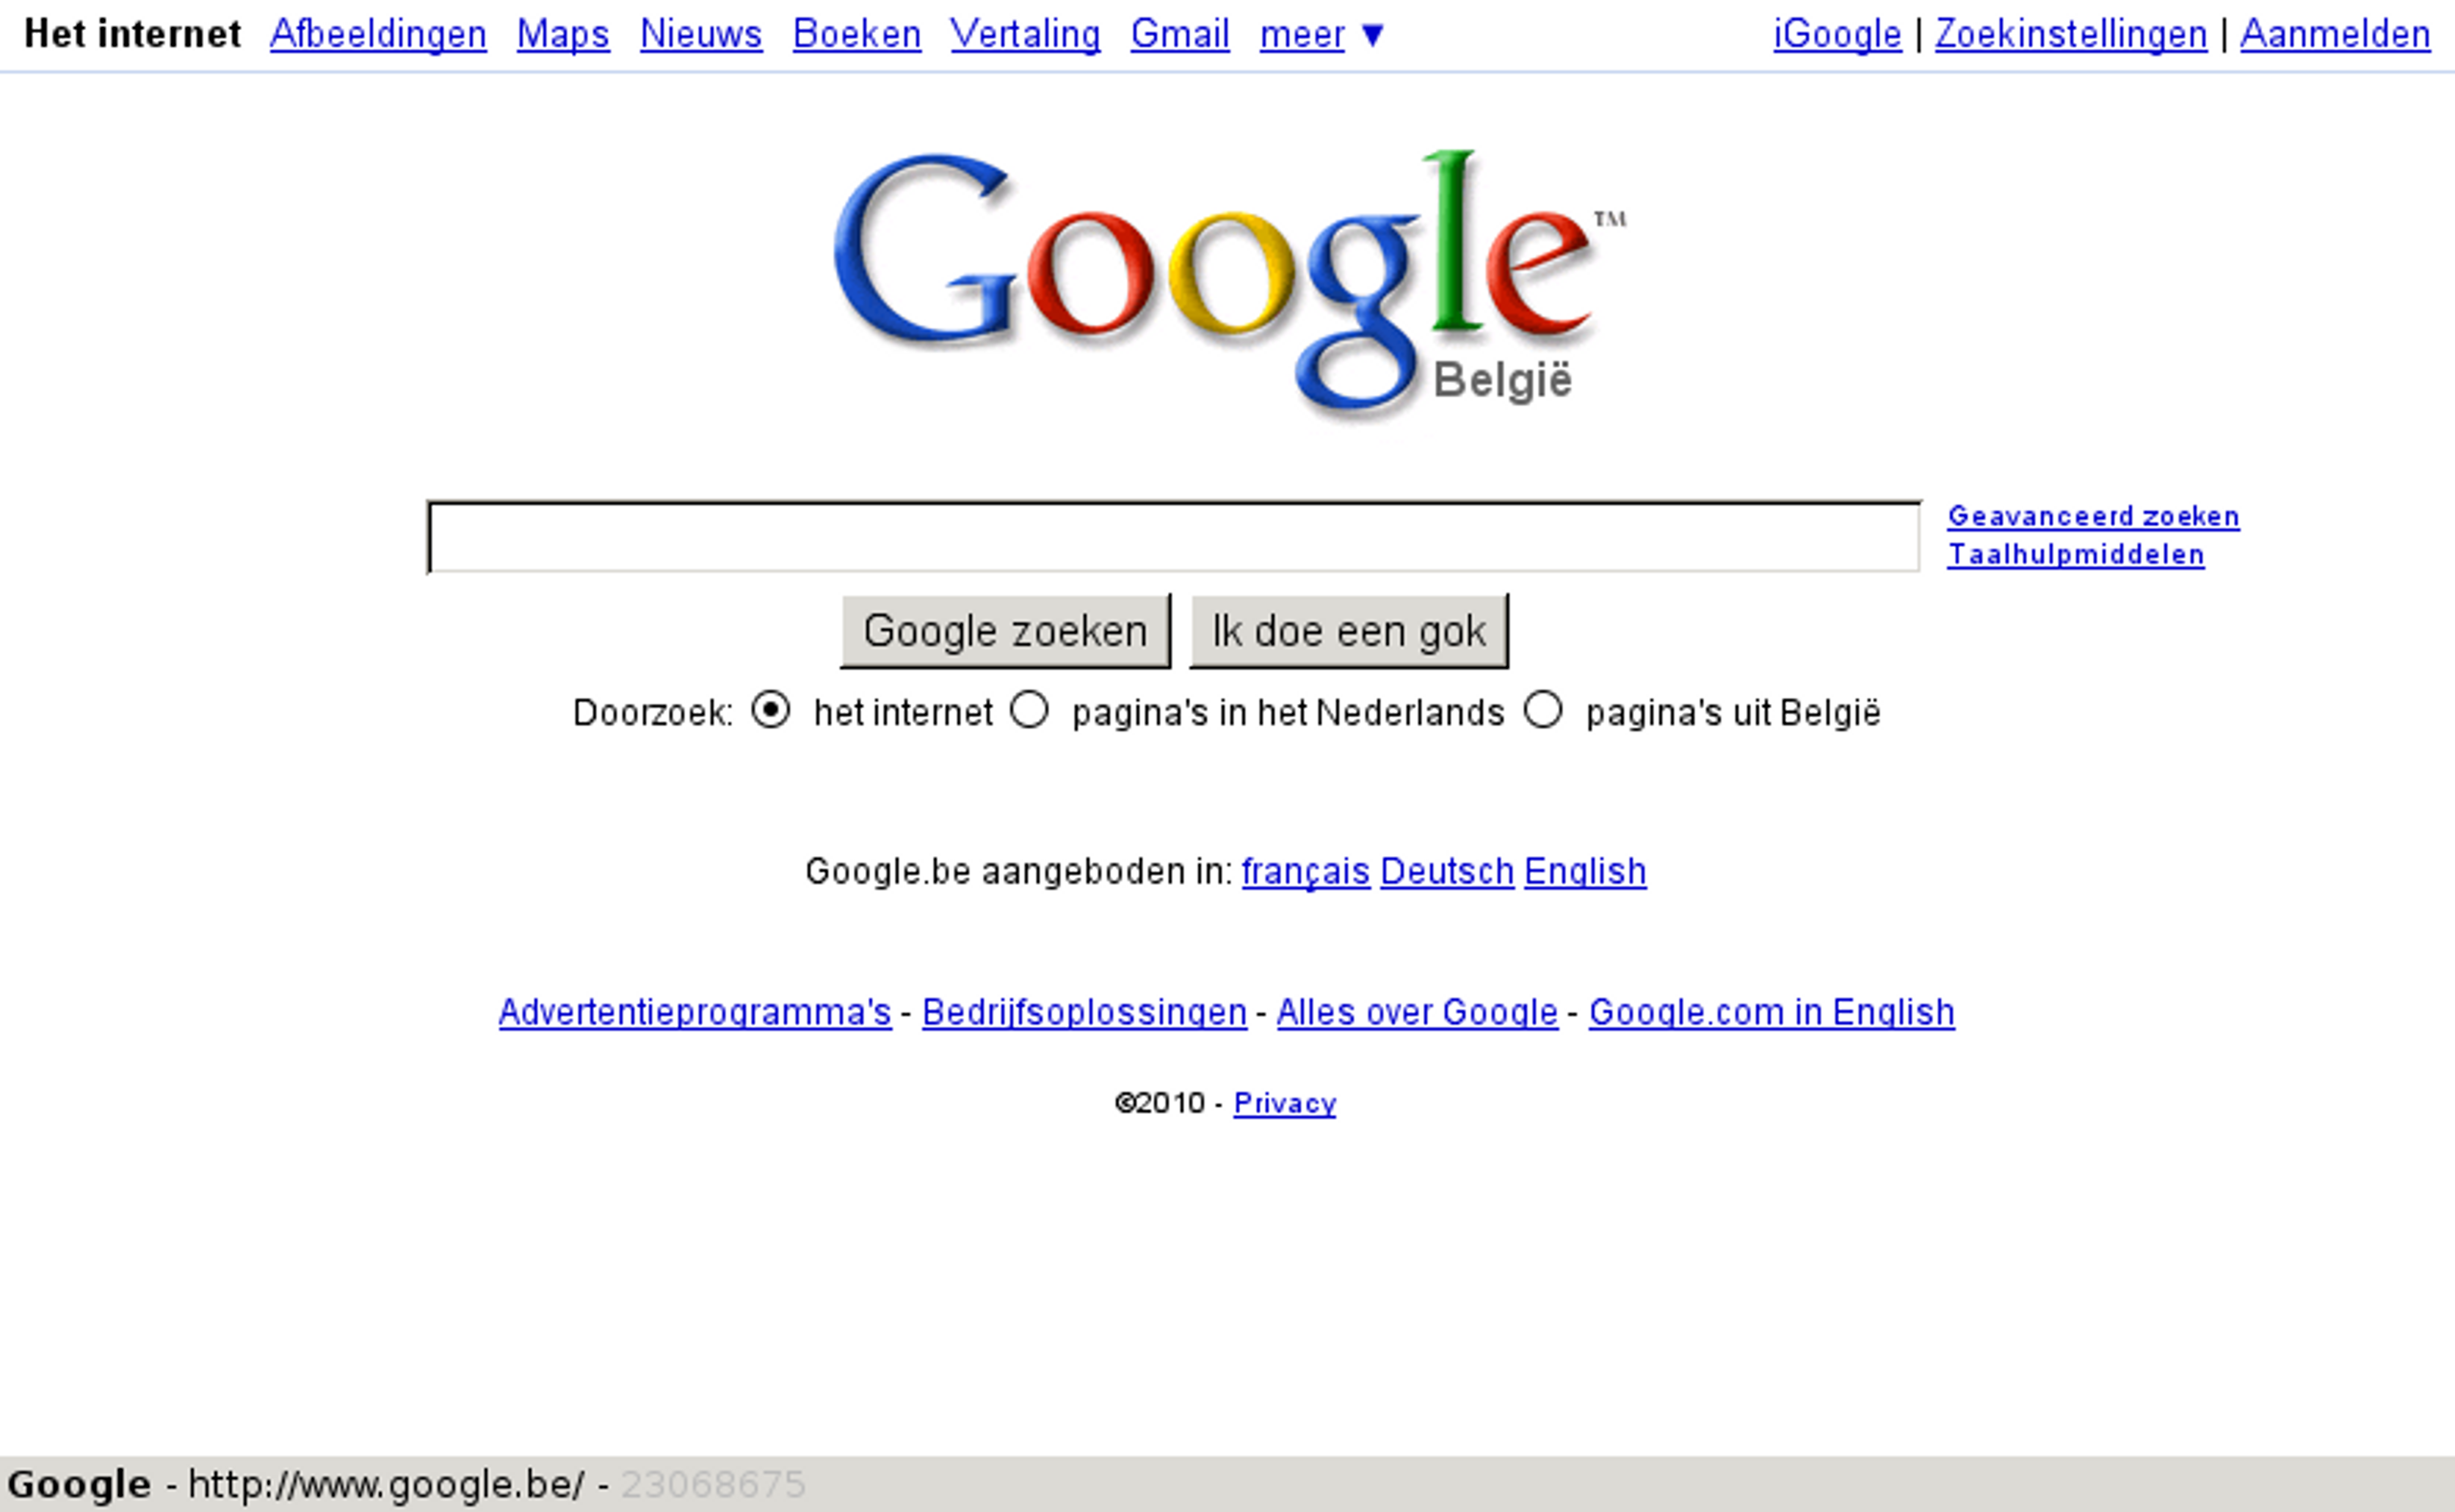
\includegraphics[scale=0.1]{uzbl-core2.png}
% -> widgets, statusbar pango, i/o
}

\frame
{ % note that this is a bit of a simplification. there are some exceptions.
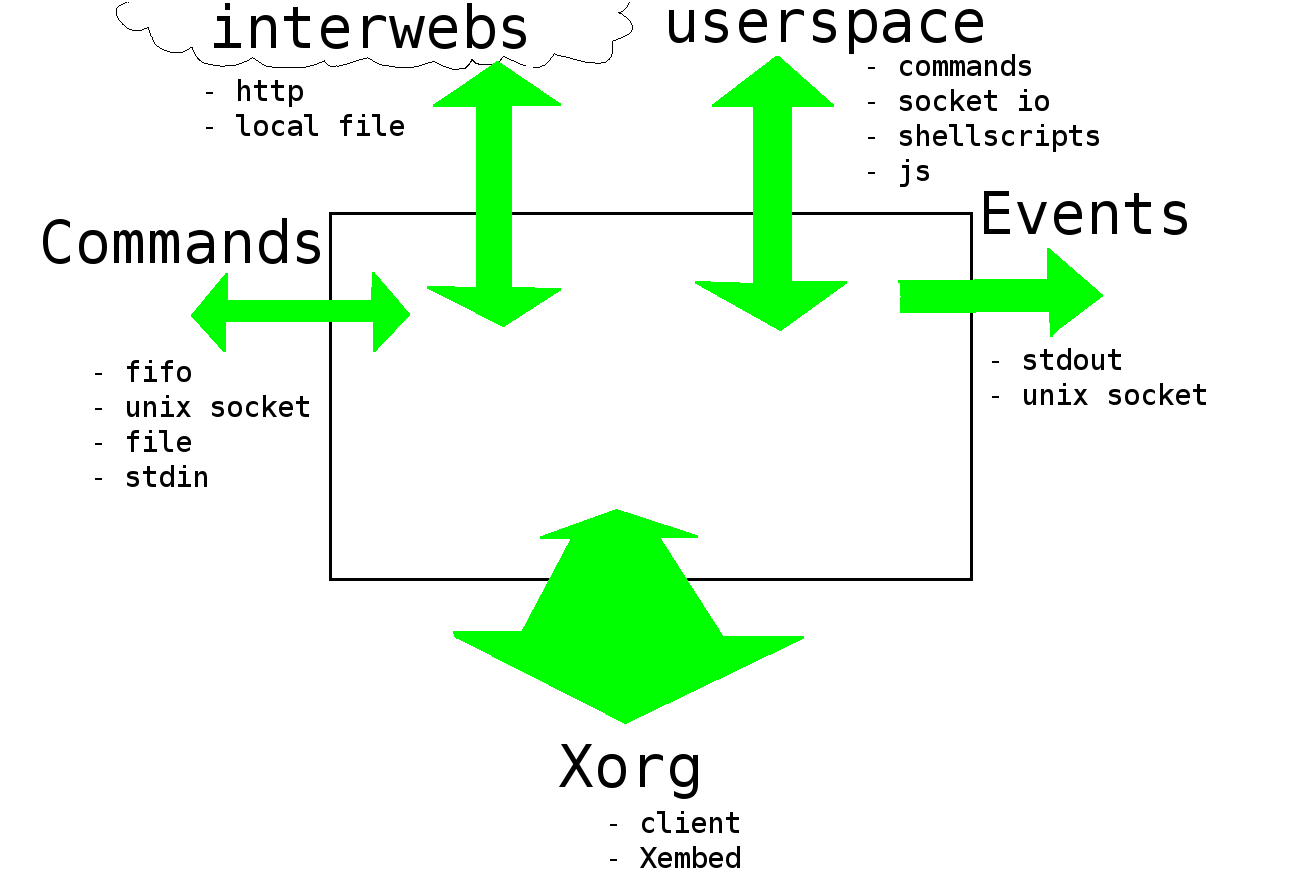
\includegraphics[scale=0.35]{uzbl-core-io.png}
% commands: change behavior/state, perform action, query information
% events: the opposite: reports anytime anything happens -> event manager
% interaction with webpages and with your system, on behalf of you.
% X obviously
}

\frame
{
\frametitle{Uzbl-core command examples}
\begin{itemize}
	\Large
	\item uri \textit{uri}
	\item reload
	\item zoom\_in
	\item spawn \textit{command}
        \item event \textit{name args} %your own custom events
\end{itemize}
}

\frame
{
\frametitle{Uzbl-core event examples}
\begin{itemize}
\Large
\item DOWNLOAD\_REQUEST \textit{uri}
\item LOAD\_PROGRESS \textit{percentage}
\item FORM\_ACTIVE
\item GEOMETRY\_CHANGED \textit{WxH+Xpos+Ypos}
\item KEY\_PRESS \textit{key/button} % note this
\end{itemize}
}


\section{Uzbl-browser}
\frame
{
\frametitle{Uzbl-browser}
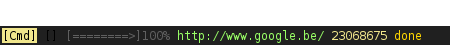
\includegraphics[scale=0.8]{uzbl-browser-statusbar.png}
% visually, the same thing. adds some things to statusbar by default.
% most of the stuff is not visual.
}

\frame
{
\frametitle{Uzbl-browser features}
  \begin{itemize} %go over them fast
\large
  \item config file
  \pause
  \item event manager %python, socket. most of the stuff below are plugins
% button/keybinds, % stacked, modkeys, modes, mode-dependent, arguments (keywords)
  \item EM plugins: bind, mode, keycmd, completion, progressbar
  \pause
  \item handlers: downloads, authentication, cookies, schemes % explain schemes
  \pause
  \item history \& bookmarks
  \pause
  \item yanking \& pasting %xclip 
  \pause
  \item forms: auto filling \& editing with external editor
  \pause
  \item page search \& zooming 
  \pause
  \item link hinting
  \pause
  \item and more..
  \end{itemize}
}


\begin{frame}[fragile]
\frametitle{History}
\large
Writing the entries:
% variable expansion tricks etc
\begin{lstlisting}
set on_event        = event ON_EVENT
@on_event LOAD_FINISH spawn @scripts_dir/history.sh
\end{lstlisting}  
\begin{lstlisting}
file=$XDG_DATA_HOME/uzbl/history
echo `date +'%Y-%m-%d %H:%M:%S'`" $6 $7" >> $file
\end{lstlisting}
\pause
Picking an entry:
\begin{lstlisting}
@cbind U = spawn @scripts_dir/load_url_from_history.sh
\end{lstlisting} 
\begin{lstlisting}
file=$XDG_DATA_HOME/uzbl/history
goto=`tac $file | dmenu | cut -d ' ' -f 3`
echo "uri $goto" > $4
\end{lstlisting}
\end{frame}

\begin{frame}[fragile]
\frametitle{Uzbl-browser history}
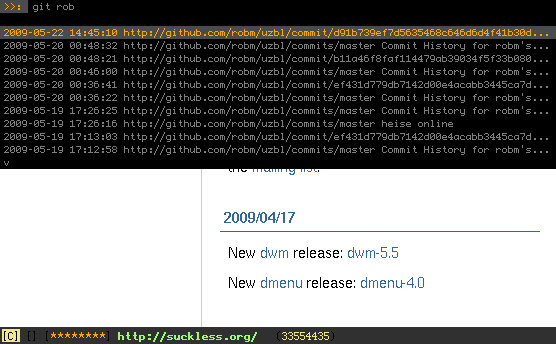
\includegraphics[scale=0.6]{history.png} % uses dmenu to load from textfile. (patched version)
\end{frame}




\begin{frame}[fragile]
\frametitle{Uzbl-browser link hinting}
\begin{lstlisting}
@cbind fl* = script @scripts_dir/follow.js '@follow_keys %s'
\end{lstlisting}
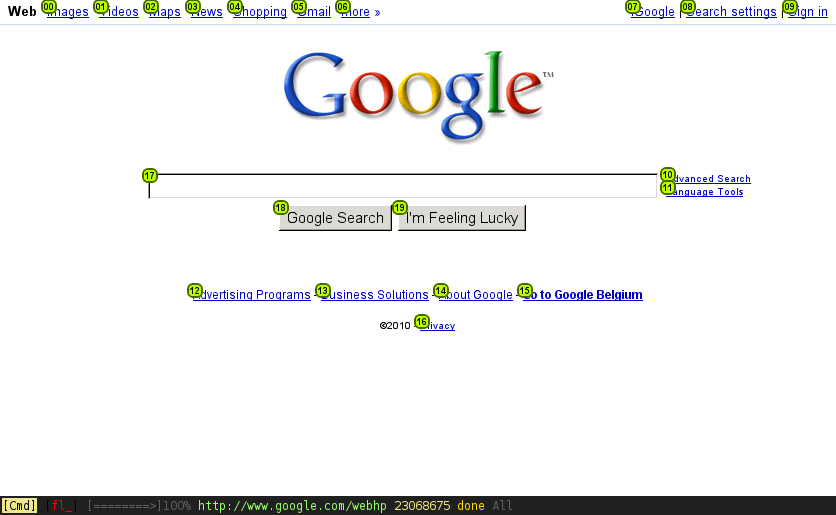
\includegraphics[scale=0.4]{uzbl-browser-follower.png}
\end{frame}



\section{Uzbl-tabbed}
% uses Xembed, do actions with uzbl events
\frame
{
\frametitle{Uzbl-tabbed}
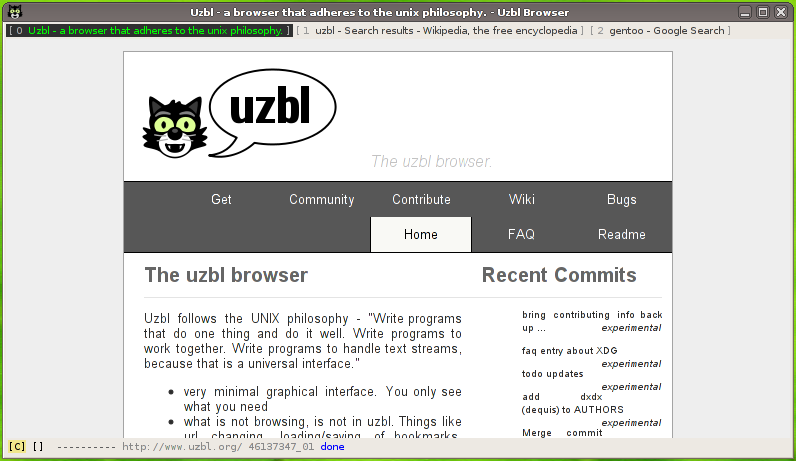
\includegraphics[scale=0.4]{uzbl-tabbed.png} % notice the Gtk bar at the top
}

\frame
{
\frametitle{Uzbl-tabbed}
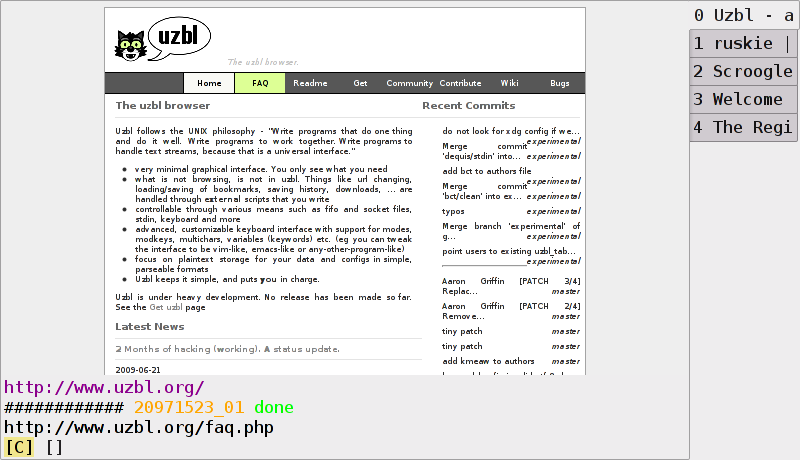
\includegraphics[scale=0.4]{uzbl-tabbed2.png} % gtk buttons. we want to abstract this so you can build tree structures etc
}

\subsection {Examples} % if there is time..

\frame
{
\frametitle{Example: Dynamic zooming}
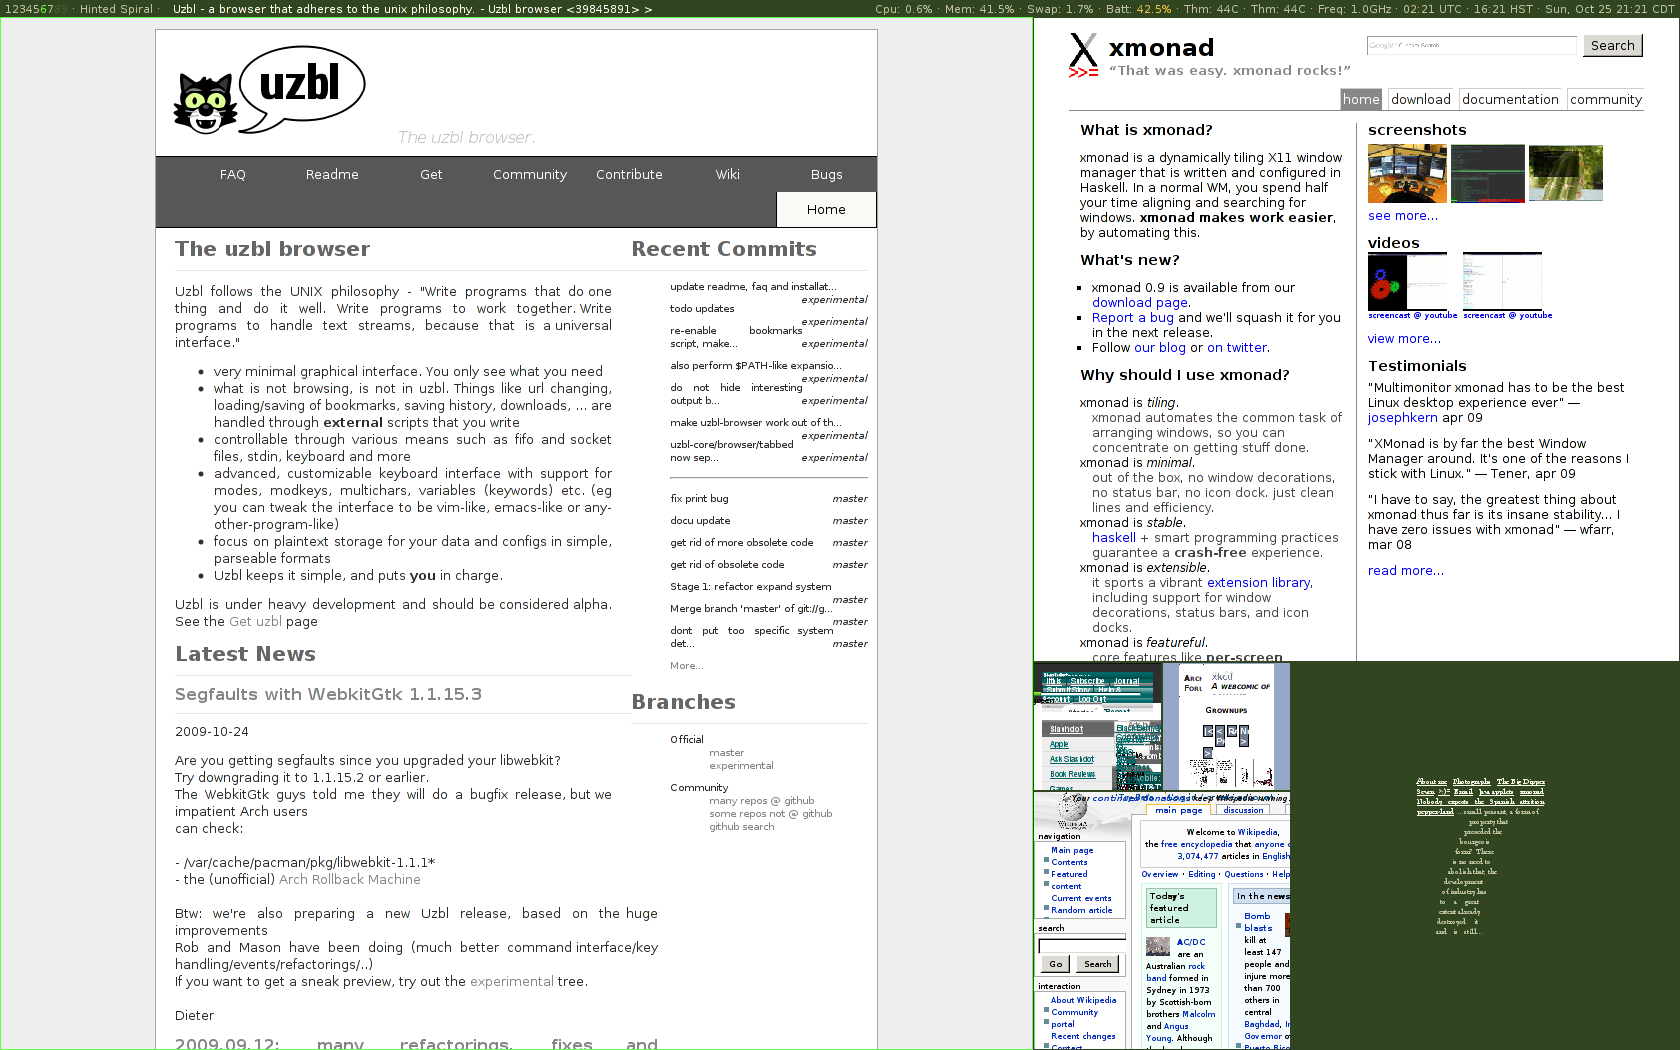
\includegraphics[scale=0.2]{dynzoom.png}
}

\begin{frame}[fragile]
\frametitle{Example: Adding a bookmark, external script}
\begin{lstlisting}
@cbind B = spawn @scripts_dir/insert_bookmark.sh
\end{lstlisting}
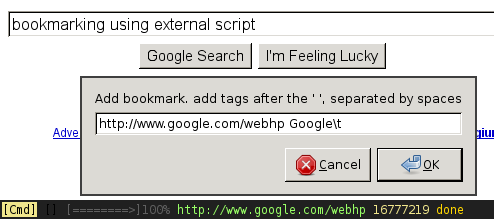
\includegraphics[scale=0.6]{bookmark-script-statusbar.png}  
\end{frame}

\begin{frame}[fragile]
\frametitle{Example: Adding a bookmark, builtin way}
\begin{lstlisting}
@cbind <Ctrl>b<tags:>_ = sh 'echo -e "$6 %s" >> $file'
\end{lstlisting}
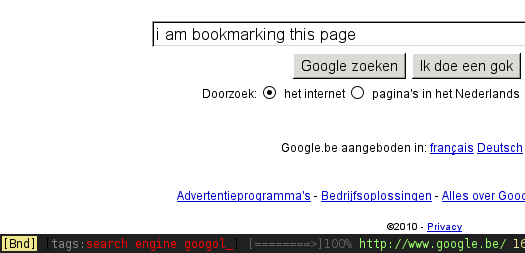
\includegraphics[scale=0.6]{bookmark-builtin-statusbar.png}
\end{frame}

\subsection{End}
\frame
{
\LARGE
\begin{center}www.uzbl.org/fosdem2010\end{center}
}

\end{document}

% more interesting things i could show but probably have no time: 
% url changing
% statusbar updating, listing uzbl instances for integration
% in WM (script for awesome?), sessions
% screensohs ezbl, xmonad tabs., C tabber, treetab
% download script, explain you want integration download manager to upload to server etc
% yanking/pasting bindings
% evt g inc/up/next maar das complicated js code.

%@bind  <Button2>  = sh 'if [ "\@SELECTED_URI" ]; then uzbl-browser -u "\@SELECTED_URI"; else echo "uri $(xclip -o)" > $4; fi'
% evt delicious thing van  http://ifacethoughts.net/2009/06/01/uzbl-the-stripped-down-browser/